\chapter{An investigation into the relationship between preoperative clinico-pathological characteristics and post-operative systemic inflammatory response in patients undergoing pancreaticoduodenectomy.}
\label{ch_pre_post_sirs}

\lhead{Chapter \ref{ch_pre_post_sirs}. \emph{Factors affecting post-operative systemic inflammation}} % This is for the header on each page - perhaps a shortened title

\clearpage
%----------------------------------------------------------------------------------------

\section{Introduction}
The perioperative systemic inflammatory response has a significant role in determining short-term and long-term outcomes following potentially curative surgery for a wide variety of cancers. Systemic inflammation both before and after major surgery has been reported to be associated with significant morbidity. 

An exaggerated preoperative systemic inflammatory response syndrome is associated with increased complications after colorectal surgery \parencite{moyes_preoperative_2009, kubo_elevated_2013}, oesophagectomy \parencite{vashist_glasgow_2010} as well as liver surgery for colorectal metastases \parencite{neal_preoperative_2011}. 
The modified Glasgow Prognostic Score in particular, which uses the combination of C-reactive protein and serum albumin, has been reported to be associated with increased incidence of complications \parencite{moyes_preoperative_2009, mohri_correlation_2014, vashist_glasgow_2010}.
Preoperative CRP levels have also been reported to be associated with increased incidence of complications including infections and renal dysfunction as well as increased in-hospital mortality after cardiac surgery \parencite{lorenzo_increased_2012, mezzomo_preoperative_2011, kim_predictive_2009, biancari_preoperative_2003, boeken_increased_1998}.

Moreover, an exaggerated postoperative systemic inflammatory response in the first few days after surgery is associated with increased incidence of infective complications after a wide variety of thoraco-abdominal procedures\parencite{platt_c-reactive_2012, dutta_persistent_2011, welsch_persisting_2008} as well as other types of surgery\parencite{mcneer_early_2010, laporta_baez_c-reactive_2011}.
The magnitude of this postoperative inflammatory response has also been reported to be associated with the severity of the complications \parencite{mcsorley_postoperative_2015}. 

In patients undergoing pancreaticoduodenectomy, preoperative systemic inflammation may be affected by several factors. 
These include the presence of obstructive jaundice with or without cholangitis, preoperative biliary intervention including endoscopic retrograde cholangio-pancreatography for diagnosis or biliary drainage and in some patients acute or chronic pancreatitis either due to obstruction of the main pancreatic duct or due to other causes. 
The effect this `priming' of the immune system on postoperative outcomes is poorly understood in this cohort of patients. 

Chronic inflammation is a recognised feature of obesity which is increasingly common in patients undergoing major surgery for pancreatic and other gastro-intestinal cancers. 
The impact of obesity, especially visceral obesity, on complications after pancreaticoduodenectomy remains controversial with some authors reporting that obesity is associated with increased incidence of complications \parencite{house_preoperative_2008, ramsey_body_2011} while others reporting similar outcomes in obese and non-obese patients \parencite{khan_does_2010, tsai_impact_2010, balentine_obesity_2011}. 

More recently, levels of adipocytokines, inflammatory mediators produced exclusively in adipose tissue, have been reported to be associated with postoperative surgical site infections after colorectal \parencite{ortega-deballon_preoperative_2013, matsuda_preoperative_2009} and gastric cancer surgery \parencite{yamamoto_association_2013}.
This emphasises the importance of adipose tissue metabolism and body composition in the preoperative systemic inflammatory status of the patient undergoing surgery. 

To our knowledge, the relationship between the preoperative systemic inflammatory response and the magnitude of the postoperative systemic inflammatory response has not been examined before. 
While obstructive jaundice in itself has recently been reported to have no effect on postoperative complications, the impact of preoperative obstructive jaundice on postoperative systemic inflammation has not been reported before. 
Moreover, the relationship between comorbidity, body composition and aerobic capacity as measured by cardiopulmonary exercise testing and postoperative systemic inflammation has not been studied. 

The aim of this study was to examine the relationship between patient factors including preoperative systemic inflammation, obstructive jaundice, cardiopulmonary exercise test parameters and body composition and the magnitude of the postoperative systemic inflammation during the first week after a pancreaticoduodenectomy. 

%Post-operative CRP levels have been reported to be associated with the magnitude of surgery as well as to predict infectious complications after neurosurgery \parencite{al-jabi_value_2010}. 


\section{Methods}
Patients who underwent elective pancreaticoduodenectomy between January 2008 and July 2012 at the West of Scotland Pancreatic Unit at the Glasgow Royal Infirmary were included in this study. 
Patients who underwent only a trial dissection or palliative surgical bypass for unresectable disease during this period were excluded.

Routine preoperative blood tests including full blood count, liver function tests and serum C-reactive protein were performed in all patients on the day before surgery. 
These blood tests were also repeated every day for at least the first postoperative week. 
These results were collected from the hospital laboratory database using an automated MS Access application as outlined in Appendix \ref{AppendixAccessDatabase}. 
The modified Glasgow Prognostic Score (mGPS) was calculated as shown in Table \ref{table:mGPS} on p\pageref{table:mGPS} in Chapter \ref{ch_intro}. 
The neutrophil-lymphocyte ratio was calculated by dividing the preoperative neutrophil count by the preoperative lymphocyte count and a threshold of 5.0 was used to dichotomise this variable. 
Standard thresholds were used to categorise other biochemical parameters. 
Obstructive jaundice was defined as serum bilirubin $>$35 $\mu$mol/L while severe obstructive jaundice was defined as serum bilirubin $>$250 $\mu$mol/L. 

Body Mass Index (BMI) was categorised using the World Health Organisation thresholds as shown in Table \ref{table:bmi_who} on p\ref{table:bmi_who} in Chapter \ref{ch_intro}. 
Only one patient had a BMI less than 18.5 kg/m$2$ and was excluded from analysis involving BMI.
The Scottish Index of Multiple Deprivation (SIMD) Quintile Scores were calculated from the post-code of the patient's primary residence and dichotomised into two groups with scores of 1-3 and 4-5 respectively.
The POSSUM Physiology Score was calculated based on 11 physiological parameters (cardiac disease including hypertension, ischaemic heart disease and heart failure, respiratory disease causing breathlessness on exertion and COPD, ECG changes, pulse rate, blood pressure, haemoglobin, white cell count, serum sodium, serum potassium, serum urea and Glasgow Coma Scale) as described in Table \todo{Create a table for PPS in introduction and reference it wherever necessary}.


In patients who underwent cardiopulmonary exercise testing, $\dot{V}_{O_2}$AT and $\dot{V}_{O_2}$Peak were compared against postoperative systemic inflammation. 
$\dot{V}_{O_2}$AT was dichotomised using a value of 10 mls/kg/min while $\dot{V}_{O_2}$Peak was dichotomised using a value of 16 mls/kg/min. 
Cardiopulmonary exercise testing methodology has been described in Section \ref{sec:cpx_method}.

Body composition was calculated in a subset of these patients using preoperative computed tomography of the abdomen. 
The methodology used in the calculation of the individual components of body composition including visceral fat, subcutaneous fat and skeletal muscle is described in detail in Section \ref{sec:bodycomp_calculation}. 
%Check this with Donny
Continuous data were converted into categorical data using tertiles.

\subsection{Statistics}

Continuous variables are reported as median (inter-quartile range).
Non-parametric tests were used to compare postoperative inflammatory markers (continuous data) with preoperative clinico-pathological characteristics (categorical data). 
Mann-Whitney U test was used when two categories were present and Kruskal-Wallis test was used when more than two categories were present.

Line-plots were created comparing the trend of inflammatory markers during the first postoperative week with preoperative systemic inflammation, obstructive jaundice and $\dot{V}_{O_2}$AT with error bars representing 95\% confidence intervals. 

SPSS software (Version 22.0; IBM, USA) was used to perform statistical analysis. Effects were considered significant at $\alpha \leq0.05$. 

\section{Results}

Pancreaticoduodenectomy was performed in 188 patients (126 male, 67\%) during the study period.
Preoperative C-reactive protein was elevated in 70 (37.6\%) patients while just over half the patients had a low preoperative serum albumin (96, 51.1\%). 
The modified Glasgow Prognostic Score revealed normal preoperative systemic inflammatory status (mGPS = 0) in 116 (62.4\%) patients, mildly systemic inflammation in 16 (8.6\%) and severe inflammation in 54 (29.0\%) patients. 
Obstructive jaundice was present in 44 (23.4\%) patients and severe obstructive jaundice was present in 31 (16.5\%) of patients. 
BMI data was available in 167 patients. More than half of these patients were overweight or obese with a BMI $>$ 25 in 87 (52.1\%) patients.

Cardiopulmonary exercise testing was performed in 130 patients. 
$\dot{V}_{O_2}$AT could not be estimated in one patient.
$\dot{V}_{O_2}$AT was less than 10 ml/kg/min in 52 (40\%) of patients indicating reduced aerobic capacity in these patients.
All the variables necessary for calculation of the POSSUM Physiology Score, a composite score of comorbidity and preoperative biochemistry, were available in 180 patients and it was elevated in 87 (48.3\%) patients.

The relationship between preoperative clinico-pathological characteristics and postoperative C-reactive protein levels (median, IQR in Table \ref{table:sirs_crp}, p-values in Table \ref{table:sirs_crp_pvalues}), postoperative serum albumin (median, IQR in Table \ref{table:sirs_alb}, p-values in Table \ref{table:sirs_alb_pvalues}), postoperative total white cell count (median, IQR in Table \ref{table:sirs_wcc}, p-values in Table \ref{table:sirs_wcc_pvalues}) and postoperative differential neutrophil count (median, IQR in Table \ref{table:sirs_neut}, p-values in Table \ref{table:sirs_neut_pvalues}) are presented.

The relationship between preoperative CRP and postoperative systemic inflammation is also depicted graphically in Fig. \ref{fig:sirs_crp}. 
The median CRP levels on the day of surgery and the first postoperative day (POD) were significantly higher in patients who had an elevated preoperative CRP. 
However, this association was not present after the first postoperative day.
Elevated preoperative CRP was associated with a persistently lower serum albumin level for the entire duration of the first postoperative week (p$<$0.001 to p$<$0.002).
It was also associated with a higher total white cell count (p$<$0.01) and higher differential neutrophil count (p$<$0.01) from the 3$^{rd}$ to 6$^{th}$ postoperative days with a less but still significant association on the 7$^{th}$ postoperative day. 

Preoperative hypoalbuminemia on the other hand was associated with lower median postoperative CRP levels starting with POD 3. 
The median difference in postoperative CRP increased from 30 mg/dl on POD 3 (p$<$0.045) to 53 mg/dl by POD 6 (p=0.002) with patients with hypoalbuminemia having a lower CRP. 
This relationship is shown in Fig. \ref{fig:sirs_alb_crp}.
Preoperative hypoalbuminemia persisted postoperatively throughout the first week (p$<$0.001, Fig. \ref{fig:sirs_alb_alb}).
There was no relationship between preoperative serum albumin levels and postoperative white cell count (Fig. \ref{fig:sirs_alb_wcc}) or neutrophil count (Fig. \ref{fig:sirs_alb_neut}).

Obstructive jaundice was associated with significant differences in the postoperative systemic inflammatory response. 
Postoperative serum albumin levels were lower in jaundiced patients and with the severely jaundiced patients having the lowest levels (p$<$0.001, Fig. \ref{fig:sirs_bil_alb}). 
There were no significant changes in the trends of albumin levels and it is likely that preoperative hypoalbuminemia persisted postoperatively in these patients. 

However, the trends in postoperative CRP were significantly different between the jaundiced and non-jaundiced patients. 
Obstructive jaundice was associated with a significantly lower peak CRP on POD 2 (p=0.001) and this persisted until POD 6 (p=0.005, Table \ref{table:sirs_crp}, \ref{table:sirs_crp_pvalues}).
Median postoperative CRP had an inverse relationship with severity of preoperative obstructive jaundice (Fig. \ref{fig:sirs_bil_crp}).
Obstructive jaundice was also associated with a delayed rise in the white cell count and neutrophil count on POD 6 (p$<$0.05) and POD 7 (p$<$0.05) although these relationships were less significant (Fig. \ref{fig:sirs_bil_wcc} and Fig. \ref{fig:sirs_bil_neut}). 

There was no significant relationship between $\dot{V}_{O_2}$AT, $\dot{V}_{O_2}$Peak and postoperative CRP, white cell count or neutrophil count. 
Serum albumin levels were lower in patients with $\dot{V}_{O_2}$AT$<$10 mls/kg/min (Fig. \ref{fig:sirs_at}).

There was no significant and persistent relationship between postoperative CRP, white cell count and neutrophil count and preoperative neutrophil-lymphocyte ratio, SIMD score, body mass index, preoperative haemoglobin levels or the POSSUM Physiology score. 
However, postoperative hypoalbuminemia was associated with all the preoperative characteristics studied with the exception of BMI and SIMD (Table \ref{table:sirs_alb} and Table \ref{table:sirs_alb_pvalues}).


\begin{sidewaystable}[p]
	\caption{The relationship  between postoperative CRP and preoperative clinico-pathological characteristics in patients undergoing pancreaticoduodenectomy. }
	\label{table:sirs_crp}
	\footnotesize
	\centering
	\renewcommand{\arraystretch}{1.2} %Increases space between rows
	%\setlength{\tabcolsep}{9pt} %sets the space between columns

	\begin{tabular}{|llr | cccccccc|}
		\hline
		Preop.              &           &   n &                                   \multicolumn{8}{c|}{Postoperative C-Reactive Protein}                                   \\
		variable            &           & 188 & Day 0      &     Day 1     &     Day 2     &     Day 3     &     Day 4     &     Day 5     &    Day 6     &     Day 7     \\ \hline
		CRP                 & $\leq$10  & 116 & 18 (11-31) & 115 (86-145)  & 214 (166-262) & 181 (132-245) & 142 (85-216)  & 114 (60-193)  & 109 (56-175) & 103 (55-175)  \\
		                    & $>$10     &  70 & 39 (26-56) & 151 (99-186)  & 211 (158-282) & 195 (145-252) & 152 (89-231)  & 114 (61-197)  & 105 (55-162) & 109 (50-172)  \\
		Albumin             & $\geq$35  &  92 & 25 (13-39) & 126 (95-157)  & 220 (165-279) & 205 (151-276) & 170 (103-241) & 131 (83-227)  & 140 (71-204) & 124 (72-192)  \\
		                    & $<$35     &  96 & 26 (14-44) & 119 (87-166)  & 204 (161-253) & 175 (124-237) & 134 (83-209)  & 101 (47-155)  & 87 (44-159)  &  88 (41-151)  \\
		mGPS                & 0         & 116 & 18 (11-31) & 115 (86-145)  & 214 (166-262) & 181 (132-245) & 142 (85-216)  & 114 (60-193)  & 109 (56-175) & 103 (55-175)  \\
		                    & 1         &  16 & 34 (25-72) & 164 (130-185) & 279 (196-304) & 229 (179-309) & 194 (128-281) & 164 (112-283) & 133 (77-226) & 127 (72-226)  \\
		                    & 2         &  54 & 39 (27-53) & 145 (95-186)  & 200 (152-248) & 179 (124-241) & 140 (79-216)  & 102 (58-153)  & 96 (54-159)  & 109 (44-154)  \\
		NLR                 & $\leq$5   & 159 & 24 (13-38) & 121 (88-161)  & 218 (165-270) & 186 (136-258) & 148 (85-226)  & 115 (60-197)  & 113 (56-175) & 117 (57-176)  \\
		                    & $>$5      &  29 & 43 (19-66) & 141 (95-167)  & 189 (152-232) & 160 (124-236) & 141 (92-189)  & 113 (67-144)  & 89 (54-149)  &  89 (50-119)  \\
		Bilirubin           & $\leq$35  & 113 & 25 (13-41) & 131 (95-165)  & 231 (180-275) & 204 (154-273) & 171 (102-237) & 127 (81-218)  & 121 (72-192) & 113 (71-175)  \\
		                    & 36-250    &  44 & 24 (14-43) & 124 (100-167) & 212 (167-277) & 182 (139-239) & 136 (90-203)  & 110 (51-139)  & 113 (48-163) & 103 (44-174)  \\
		                    & $>$250    &  31 & 28 (17-37) &  99 (67-128)  & 165 (116-202) & 149 (82-214)  &  95 (60-166)  &  59 (37-153)  & 55 (26-154)  &  70 (24-158)  \\
		BMI                 & $<25$     &  80 & 21 (12-42) & 121 (88-163)  & 207 (156-252) & 174 (132-242) & 134 (86-217)  & 105 (58-193)  & 87 (51-175)  &  92 (50-164)  \\
		                    & 25-29.9   &  64 & 26 (17-39) & 127 (93-164)  & 220 (187-269) & 203 (137-250) & 149 (86-201)  & 115 (62-164)  & 109 (55-165) & 110 (54-170)  \\
		                    & 30-34.9   &  23 & 34 (12-42) & 114 (90-133)  & 220 (148-270) & 205 (152-287) & 190 (97-230)  & 141 (67-222)  & 142 (55-181) & 136 (70-198)  \\
		                    & $>$35     &   9 & 31 (27-44) & 167 (116-178) & 204 (173-311) & 235 (147-293) & 210 (91-290)  & 167 (76-232)  & 172 (88-207) & 162 (148-178) \\
		%bmi                & $\leq$25  &  80 & 21 (12-42) & 121 (88-163)  & 207 (156-252) & 174 (132-242) & 134 (86-217)  & 105 (58-193)  & 87 (51-175)  &  92 (50-164)  \\
		%                   & $>$25     &  96 & 27 (17-40) & 124 (93-162)  & 220 (170-270) & 205 (148-266) & 164 (90-217)  & 118 (66-192)  & 117 (57-172) & 122 (57-175)  \\
		SIMD                & 4-5       &  61 & 26 (13-45) & 128 (98-168)  & 226 (183-271) & 208 (150-274) & 171 (108-231) & 127 (88-200)  & 137 (72-205) & 136 (71-220)  \\
		                    & 1-3       & 126 & 25 (14-39) & 121 (88-161)  & 207 (148-264) & 180 (132-242) & 140 (84-215)  & 105 (57-190)  & 94 (50-163)  &  98 (50-158)  \\
		$\dot{V}_{O_2}$AT   & $\geq$10  &  77 & 23 (12-40) & 118 (85-165)  & 222 (166-264) & 186 (132-252) & 148 (85-231)  & 111 (58-193)  & 106 (54-177) & 107 (51-173)  \\
		                    & $<$10     &  52 & 28 (19-41) & 121 (96-150)  & 222 (158-275) & 204 (151-262) & 175 (123-221) & 119 (80-204)  & 116 (63-174) & 113 (66-189)  \\
		$\dot{V}_{O_2}$Peak & $\geq$16 &  65 & 21 (12-37) & 106 (78-150)  & 214 (140-264) & 181 (132-235) & 150 (85-213)  & 110 (59-190)  & 113 (57-181) & 115 (51-175)  \\
		                    & $<$16     &  65 & 28 (19-44) & 123 (100-161) & 234 (173-279) & 214 (149-278) & 174 (92-237)  & 119 (63-204)  & 111 (57-172) & 111 (60-180)  \\
		Hb                  & $\geq$12  & 127 & 24 (13-38) & 116 (85-161)  & 214 (165-263) & 184 (136-247) & 151 (88-214)  & 111 (59-192)  & 102 (54-172) & 104 (51-174)  \\
		                    & $<$12     &  61 & 28 (18-45) & 140 (104-165) & 216 (163-279) & 186 (124-258) & 137 (89-231)  & 119 (64-197)  & 119 (63-170) & 106 (60-170)  \\
		PPS                 & $\leq$14  &  93 & 24 (13-36) & 116 (84-161)  & 205 (144-264) & 180 (129-242) & 131 (83-210)  & 107 (55-168)  & 104 (54-174) & 104 (52-174)  \\
		                    & $>$14     &  87 & 26 (14-45) & 128 (99-156)  & 214 (175-262) & 198 (136-255) & 158 (95-226)  & 118 (71-193)  & 114 (58-167) & 109 (53-173)  \\ \hline
	\end{tabular}	
\end{sidewaystable}
































\begin{sidewaystable}[p]
	\caption{The relationship  between postoperative Albumin and preoperative clinico-pathological characteristics in patients undergoing pancreaticoduodenectomy. }
	\label{table:sirs_albumin}
	\footnotesize
	\centering
	\renewcommand{\arraystretch}{1.2} %Increases space between rows
	%\setlength{\tabcolsep}{9pt} %sets the space between columns

	\begin{tabular}{|llr | c c c c c c c c|}
		\hline
		Preop.              &           & n   &                           \multicolumn{8}{c|}{Postoperative Serum Albumin}                            \\
		variable            &           & 188 & Day 0      & Day 1      & Day 2      & Day 3      & Day 4      & Day 5      & Day 6      & Day 7      \\ \hline
		CRP                 & $\leq$10  & 116 & 19 (16-23) & 20 (18-23) & 20 (18-23) & 19 (17-22) & 20 (16-22) & 20 (17-23) & 20 (17-23) & 20 (17-24) \\
		                    & $>$10     & 70  & 16 (13-19) & 17 (14-21) & 17 (15-20) & 16 (14-19) & 16 (14-19) & 17 (15-19) & 17 (15-20) & 18 (15-22) \\
		Albumin             & $\geq$35  & 92  & 20 (18-23) & 22 (19-24) & 22 (20-23) & 20 (19-23) & 20 (18-23) & 21 (18-23) & 21 (19-24) & 21 (19-25) \\
		                    & $<$35     & 96  & 16 (13-19) & 16 (14-20) & 17 (14-19) & 16 (13-19) & 16 (14-19) & 16 (14-19) & 17 (15-20) & 17 (14-20) \\
		mGPS                & 0         & 116 & 19 (16-23) & 20 (18-23) & 20 (18-23) & 19 (17-22) & 20 (16-22) & 20 (17-23) & 20 (17-23) & 20 (17-24) \\
		                    & 1         & 16  & 20 (18-22) & 22 (19-23) & 21 (19-22) & 20 (18-22) & 19 (17-21) & 18 (17-23) & 20 (18-23) & 21 (17-24) \\
		                    & 2         & 54  & 14 (13-17) & 16 (14-18) & 16 (14-18) & 15 (13-19) & 15 (14-19) & 16 (14-18) & 16 (14-20) & 17 (14-20) \\
		NLR                 & $\leq$5   & 159 & 19 (15-22) & 20 (16-23) & 20 (17-22) & 19 (16-22) & 19 (15-22) & 19 (16-22) & 19 (16-23) & 20 (16-23) \\
		                    & $>$5      & 29  & 15 (12-18) & 17 (15-19) & 17 (15-20) & 16 (14-19) & 17 (14-19) & 17 (15-19) & 18 (16-20) & 19 (15-22) \\
		Bilirubin           & $\leq$35  & 113 & 20 (17-23) & 21 (18-24) & 21 (19-23) & 20 (18-22) & 20 (18-22) & 20 (18-23) & 20 (18-23) & 21 (18-23) \\
		                    & 36-250    & 44  & 16 (14-20) & 18 (14-21) & 17 (16-20) & 16 (15-19) & 17 (14-20) & 17 (15-22) & 18 (15-23) & 19 (15-23) \\
		                    & $>$250    & 31  & 14 (12-16) & 15 (13-17) & 15 (12-17) & 14 (12-16) & 14 (13-16) & 15 (13-17) & 15 (14-17) & 15 (13-19) \\
		BMI                 & $<25$     & 80  & 17 (14-20) & 19 (15-22) & 18 (16-22) & 18 (15-20) & 18 (15-21) & 18 (15-22) & 19 (15-22) & 19 (15-23) \\
		                    & 25-29.9   & 64  & 19 (14-21) & 20 (16-23) & 20 (16-23) & 19 (15-22) & 19 (16-21) & 19 (17-22) & 20 (17-22) & 20 (17-23) \\
		                    & 30-34.9   & 23  & 19 (16-23) & 19 (16-22) & 20 (17-22) & 19 (16-21) & 19 (16-21) & 20 (17-22) & 19 (17-22) & 20 (19-23) \\
		                    & $>$35     & 9   & 20 (17-23) & 19 (18-26) & 20 (18-22) & 19 (18-20) & 19 (17-20) & 17 (16-21) & 18 (16-20) & 18 (17-20) \\
		%bmi                & $\leq$25  & 80  & 17 (14-20) & 19 (15-22) & 18 (16-22) & 18 (15-20) & 18 (15-21) & 18 (15-22) & 19 (15-22) & 19 (15-23) \\
		%                   & $>$25     & 96  & 19 (15-22) & 19 (16-23) & 20 (17-22) & 19 (16-21) & 19 (16-21) & 19 (17-22) & 19 (17-22) & 20 (17-23) \\
		SIMD                & 1-3       & 87  & 19 (15-22) & 19 (16-23) & 20 (16-22) & 19 (15-21) & 19 (15-21) & 18 (15-21) & 19 (15-22) & 20 (15-23) \\
		                    & 4-5       & 100 & 18 (14-21) & 19 (15-22) & 19 (16-22) & 19 (16-22) & 19 (16-21) & 18 (16-22) & 19 (16-22) & 19 (16-23) \\
		$\dot{V}_{O_2}$AT   & $\geq$10  & 77  & 19 (16-23) & 20 (18-23) & 20 (18-22) & 19 (16-22) & 19 (16-21) & 19 (17-22) & 20 (17-22) & 20 (16-23) \\
		                    & $<$10     & 52  & 17 (13-20) & 18 (15-22) & 17 (15-22) & 16 (14-20) & 17 (14-21) & 17 (14-20) & 17 (14-20) & 18 (15-21) \\
		$\dot{V}_{O_2}$Peak & $\geq$160 & 65  & 20 (16-23) & 21 (17-23) & 20 (18-23) & 19 (16-22) & 19 (16-22) & 19 (17-23) & 20 (16-23) & 20 (16-23) \\
		                    & $<$16     & 65  & 18 (14-20) & 19 (15-21) & 18 (15-22) & 17 (15-20) & 18 (14-20) & 18 (15-20) & 18 (15-20) & 19 (15-22) \\
		Haemoglobin         & $\geq$12  & 127 & 19 (16-22) & 20 (17-23) & 20 (18-23) & 19 (17-22) & 19 (16-22) & 20 (17-23) & 20 (17-23) & 20 (17-24) \\
		                    & $<$12     & 61  & 16 (13-19) & 17 (14-20) & 17 (14-20) & 16 (13-19) & 16 (14-19) & 17 (14-18) & 17 (15-20) & 17 (15-21) \\
		PPS                 & $\leq$14  & 93  & 19 (16-23) & 20 (17-23) & 20 (18-23) & 19 (17-22) & 20 (16-22) & 20 (17-23) & 20 (16-23) & 21 (17-25) \\
		                    & $>$14     & 87  & 17 (14-20) & 18 (15-21) & 18 (15-21) & 16 (13-20) & 17 (14-20) & 17 (14-20) & 18 (15-22) & 19 (15-22)\\ \hline
	\end{tabular}	
\end{sidewaystable}






































\begin{table}[p]
	\caption{The relationship  between postoperative C-reactive protein and preoperative clinicopathological characteristics in patients undergoing pancreaticoduodenectomy: p-values only. }
	\label{table:sirs_crp_pvalues}
	\footnotesize
	\centering
	\renewcommand{\arraystretch}{1.2} %Increases space between rows
	%\setlength{\tabcolsep}{9pt} %sets the space between columns

	\begin{tabular}{|l | c c c c c c c c|}
		\hline
		Preop.              &         \multicolumn{8}{c|}{Postoperative C-Reactive Protein}          \\
		Variable            & Day 0    & Day 1    & Day 2 & Day 3 & Day 4 & Day 5    & Day 6 & Day 7 \\ \hline
		CRP                 & $<$0.001 & $<$0.001 & 0.669 & 0.522 & 0.741 & 0.831    & 0.789 & 0.834 \\
		Albumin             & 0.445    & 0.916    & 0.148 & 0.045 & 0.018 & 0.001    & 0.002 & 0.006 \\
		mGPS                & $<$0.001 & 0.001    & 0.037 & 0.048 & 0.084 & 0.029    & 0.215 & 0.347 \\
		NLR                 & 0.001    & 0.310    & 0.143 & 0.217 & 0.490 & 0.427    & 0.227 & 0.111 \\
		Bilirubin           & 0.869    & 0.009    & 0.001 & 0.001 & 0.003 & $<$0.001 & 0.005 & 0.072 \\
		BMI                 & 0.181    & 0.312    & 0.744 & 0.376 & 0.424 & 0.504    & 0.556 & 0.214 \\
		%BMI    01          & 0.057    & 0.910    & 0.325 & 0.135 & 0.474 & 0.375    & 0.426 & 0.166 \\
		SIMD                & 0.962    & 0.399    & 0.277 & 0.243 & 0.163 & 0.422    & 0.849 & 0.713 \\
		$\dot{V}_{O_2}$AT   & 0.042    & 0.749    & 0.838 & 0.587 & 0.330 & 0.448    & 0.659 & 0.389 \\
		$\dot{V}_{O_2}$Peak & 0.022    & 0.050    & 0.122 & 0.154 & 0.218 & 0.537    & 0.992 & 0.527 \\
		Haemoglobin         & 0.025    & 0.078    & 0.735 & 0.973 & 0.905 & 0.838    & 0.682 & 0.987 \\
		PPS                 & 0.114    & 0.192    & 0.525 & 0.308 & 0.127 & 0.338    & 0.954 & 0.919 \\ \hline
		\multicolumn{9}{l}{\textit{p} - Mann-Whitney U test or Kruskal-Wallis test}
	\end{tabular}	
	\vspace{1cm}

	
	\caption{The relationship  between postoperative serum albumin and preoperative clinicopathological characteristics in patients undergoing pancreaticoduodenectomy: p-values only. }
	\label{table:sirs_alb_pvalues}
		\begin{tabular}{|l | c c c c c c c c|}
			\hline
			Preop.              &                   \multicolumn{8}{c|}{Postoperative Serum Albumin}                    \\
			Variable            & Day 0    & Day 1    & Day 2    & Day 3    & Day 4    & Day 5    & Day 6    & Day 7    \\ \hline
			CRP                 & $<$0.001 & $<$0.001 & $<$0.001 & $<$0.001 & $<$0.001 & $<$0.001 & 0.001    & 0.002    \\
			Albumin             & $<$0.001 & $<$0.001 & $<$0.001 & $<$0.001 & $<$0.001 & $<$0.001 & $<$0.001 & $<$0.001 \\
			mGPS                & $<$0.001 & $<$0.001 & $<$0.001 & $<$0.001 & $<$0.001 & $<$0.001 & $<$0.001 & 0.001    \\
			NLR                 & $<$0.001 & $<$0.001 & 0.002    & 0.004    & 0.014    & 0.008    & 0.150    & 0.137    \\
			Bilirubin           & $<$0.001 & $<$0.001 & $<$0.001 & $<$0.001 & $<$0.001 & $<$0.001 & $<$0.001 & $<$0.001 \\
			BMI                 & 0.126    & 0.413    & 0.446    & 0.374    & 0.671    & 0.821    & 0.595    & 0.700    \\
			%BMI    01          & 0.068    & 0.153    & 0.169    & 0.116    & 0.238    & 0.378    & 0.221    & 0.406    \\
			SIMD                & 0.297    & 0.407    & 0.336    & 0.848    & 0.984    & 0.940    & 0.850    & 0.915    \\
			$\dot{V}_{O_2}$AT   & 0.020    & 0.010    & 0.024    & 0.022    & 0.012    & 0.019    & 0.024    & 0.068    \\
			$\dot{V}_{O_2}$Peak & 0.012    & 0.015    & 0.023    & 0.016    & 0.020    & 0.032    & 0.019    & 0.188    \\
			Haemoglobin         & $<$0.001 & $<$0.001 & $<$0.001 & $<$0.001 & $<$0.001 & $<$0.001 & 0.001    & 0.001    \\
			PPS                 & 0.002    & 0.001    & $<$0.001 & $<$0.001 & $<$0.001 & 0.001    & 0.019    & 0.014    \\ \hline
			\multicolumn{9}{l}{\textit{p} - Mann-Whitney U test or Kruskal-Wallis test}
		\end{tabular}
\end{table}
\begin{sidewaystable}[p]
	\caption{The relationship  between postoperative white cell count and preoperative clinico-pathological characteristics in patients undergoing pancreaticoduodenectomy }
	\label{table:sirs_wcc}
	\footnotesize
	\centering
	\renewcommand{\arraystretch}{1.2} %Increases space between rows
	\setlength{\tabcolsep}{5pt} %sets the space between columns
	
	\begin{tabular}{|l l | cc cc cc cc|}
		\hline
		Preop.              & n         &                                            \multicolumn{8}{c|}{Postoperative White Cell Count}                                             \\
		Variable            & 188       & Day 0           &      Day 1      & Day 2           &     Day 3      & Day 4          &     Day 5      & Day 6           &      Day 7      \\ \hline
		CRP                 & $\leq$10  & 11.7(9.3-14.8)  & 12.3(10.7-15.6) & 13.4(10.8-16.7) & 9.9(7.9-13.3)  & 8.9(6.4-11.4)  & 9.1(6.5-12.5)  & 10.6(8.0-14.7)  & 12.5(9.3-16.0)  \\
		                    & $>$10     & 12.5(10.2-15.6) & 14.1(11.1-17.7) & 14.9(11.9-18.3) & 12.8(9.5-15.3) & 10.3(8.0-14.1) & 11.0(8.8-13.5) & 13.4(9.9-16.6)  & 14.6(11.6-18.7) \\
		Albumin             & $\geq$35  & 12.2(9.8-14.9)  & 13.1(10.7-16.3) & 13.5(11.0-17.5) & 10.9(8.2-14.2) & 9.4(6.8-11.6)  & 9.4(7.0-12.5)  & 11.1(8.0-15.1)  & 13.3(10.0-16.4) \\
		                    & $<$35     & 12.1(9.7-15.4)  & 13.1(10.9-16.1) & 14.2(11.8-17.4) & 11.1(8.4-14.7) & 9.6(7.2-12.9)  & 10.2(8.1-13.2) & 12.6(9.4-16.0)  & 13.8(10.4-18.1) \\
		mGPS                & 0         & 11.7(9.3-14.8)  & 12.3(10.7-15.6) & 13.4(10.8-16.7) & 9.9(7.9-13.3)  & 8.9(6.4-11.4)  & 9.1(6.5-12.5)  & 10.6(8.0-14.7)  & 12.5(9.3-16.0)  \\
		                    & 1         & 12.3(10.4-15.3) & 15.1(10.4-17.4) & 15.7(11.6-18.5) & 13.0(8.8-15.4) & 10.0(6.8-13.0) & 10.1(8.2-11.7) & 12.3(9.4-15.0)  & 13.1(11.1-17.0) \\
		                    & 2         & 12.5(10.2-15.8) & 13.7(11.2-17.8) & 14.9(11.9-18.2) & 12.7(9.6-15.3) & 10.8(8.1-15.0) & 11.0(8.9-14.0) & 14.5(10.0-16.6) & 14.8(11.7-19.7) \\
		NLR                 & $\leq$5   & 12.2(9.7-14.9)  & 13.3(10.9-16.4) & 13.7(11.0-17.4) & 10.9(8.3-14.2) & 9.5(6.9-12.3)  & 9.8(7.4-13.0)  & 12.0(8.6-15.9)  & 13.6(10.1-17.6) \\
		                    & $>$5      & 11.8(10.4-15.6) & 11.9(9.5-15.1)  & 14.2(12.4-18.1) & 11.5(8.6-14.3) & 8.8(6.8-14.0)  & 9.2(8.0-12.3)  & 11.0(9.5-15.2)  & 13.2(10.5-15.3) \\
		Bilirubin           & $\leq$35  & 12.2(9.2-15.7)  & 13.2(10.6-16.3) & 13.7(10.8-17.4) & 10.9(8.2-14.0) & 9.5(6.9-12.2)  & 9.5(7.2-12.4)  & 11.0(8.6-15.2)  & 13.2(10.1-16.0) \\
		                    & 36-250    & 12.2(9.9-14.5)  & 13.7(10.9-17.5) & 13.8(11.4-17.7) & 10.4(8.4-15.1) & 8.8(6.8-12.9)  & 9.6(8.1-12.7)  & 12.2(8.9-15.9)  & 13.2(9.5-17.2)  \\
		                    & $>$250    & 12.1(10.6-14.4) & 12.9(11.1-15.1) & 14.2(11.9-17.0) & 11.8(8.3-13.8) & 10.4(7.2-12.7) & 12.3(7.8-16.5) & 15.6(11.9-17.1) & 14.7(11.9-21.0) \\
		BMI                 & $<25$     & 11.6(9.5-14.6)  & 12.5(10.5-15.3) & 13.4(10.4-17.0) & 10.2(8.3-13.8) & 9.4(7.1-12.2)  & 9.8(7.3-12.8)  & 11.5(9.1-15.6)  & 12.7(9.8-17.3)  \\
		                    & 25-29.9   & 12.8(9.6-15.7)  & 13.5(10.7-17.6) & 15.5(12.4-18.4) & 12.1(8.7-14.9) & 10.3(6.9-12.9) & 10.4(8.2-12.9) & 11.9(9.8-15.7)  & 13.6(11.0-16.4) \\
		                    & 30-34.9   & 11.5(8.7-14.5)  & 13.0(10.9-16.1) & 13.5(10.5-18.1) & 10.4(7.6-14.3) & 8.5(7.0-11.6)  &  8.1(6.5-9.8)  & 9.5(7.3-14.7)   & 12.2(8.3-16.5)  \\
		                    & $>$35     & 13.0(10.5-16.3) & 12.2(11.4-14.5) & 13.3(12.9-14.4) & 12.7(5.9-13.0) & 7.9(6.0-12.4)  & 8.8(6.9-12.8)  & 10.3(8.7-16.2)  & 15.6(11.7-20.6) \\
		%bmi                & $\leq$25  & 11.6(9.5-14.6)  & 12.5(10.5-15.3) & 13.4(10.4-17.0) & 10.2(8.3-13.8) & 9.4(7.1-12.2)  & 9.8(7.3-12.8)  & 11.5(9.1-15.6)  & 12.7(9.8-17.3)  \\
		%                   & $>$25     & 12.3(9.8-15.7)  & 13.3(10.9-17.0) & 14.6(12.2-18.2) & 11.8(8.3-14.6) & 9.5(6.9-12.7)  & 9.6(7.6-12.8)  & 11.5(8.8-15.7)  & 13.6(10.7-16.5) \\
		SIMD                & 1-3       & 12.4(10.3-15.7) & 13.0(11.1-16.3) & 13.8(11.7-18.1) & 10.4(8.2-14.3) & 9.4(6.9-11.9)  & 9.4(7.4-13.0)  & 12.0(9.2-15.9)  & 13.6(10.6-17.9) \\
		                    & 4-5       & 11.9(9.4-14.8)  & 13.2(10.2-16.2) & 13.7(10.8-17.4) & 11.2(8.3-14.2) & 9.7(6.9-13.0)  & 9.8(7.5-12.9)  & 11.5(8.7-15.7)  & 13.5(9.8-16.9)  \\
		$\dot{V}_{O_2}$AT   & $\geq$10  & 12.6(10.2-15.6) & 13.2(10.9-17.1) & 13.8(11.1-17.4) & 11.4(8.6-14.6) & 10.2(7.7-12.2) & 9.8(8.0-13.0)  & 12.6(9.7-15.9)  & 14.2(10.6-17.1) \\
		                    & $<$10     & 11.5(9.2-14.4)  & 13.4(10.1-16.3) & 14.8(10.8-17.7) & 11.4(8.3-14.6) & 9.5(7.3-12.8)  & 9.6(7.4-13.2)  & 11.6(8.5-15.9)  & 13.6(10.5-15.9) \\
		$\dot{V}_{O_2}$Peak & $\geq$160 & 12.4(9.9-14.9)  & 12.7(10.3-16.3) & 13.8(11.1-17.4) & 10.8(8.1-14.6) & 9.7(7.7-11.5)  & 9.7(7.5-12.7)  & 12.4(9.3-16.0)  & 14.0(9.8-17.6)  \\
		                    & $<$16     & 11.6(9.7-15.3)  & 13.9(10.9-16.7) & 14.7(11.0-18.0) & 11.6(9.0-14.3) & 9.9(7.6-13.0)  & 9.8(7.5-13.3)  & 12.0(8.7-15.5)  & 13.8(10.6-16.0) \\
		Hb                  & $\geq$12  & 12.1(9.4-15.6)  & 13.2(10.6-16.3) & 13.7(10.8-17.2) & 10.5(8.3-13.5) & 9.4(6.9-11.7)  & 9.6(7.5-12.7)  & 11.1(8.7-15.7)  & 13.5(10.1-17.7) \\
		                    & $<$12     & 12.1(9.9-14.5)  & 13.0(11.5-16.3) & 14.1(11.9-18.1) & 11.7(8.1-16.0) & 9.5(7.0-14.1)  & 10.5(7.4-13.2) & 12.6(9.5-15.9)  & 13.4(10.5-17.1) \\
		PPS                 & $\leq$14  & 12.2(9.9-14.7)  & 12.6(10.9-15.7) & 13.3(10.8-16.7) & 10.2(8.1-13.4) & 9.0(6.8-11.6)  & 9.6(7.2-12.6)  & 10.9(8.2-15.3)  & 13.3(9.5-17.7)  \\
		                    & $>$14     & 11.8(9.2-15.5)  & 13.0(9.9-17.2)  & 14.1(11.8-18.1) & 11.7(8.3-15.3) & 9.5(7.0-13.6)  & 10.2(7.5-13.2) & 12.4(9.4-15.9)  & 13.5(10.4-16.0) \\ \hline
	\end{tabular}	
\end{sidewaystable}

  





\begin{sidewaystable}[p]
	\caption{The relationship  between postoperative neutrophil count and preoperative clinico-pathological characteristics in patients undergoing pancreaticoduodenectomy. }
	\label{table:sirs_neut}
	\footnotesize
	\centering
	\renewcommand{\arraystretch}{1.2} %Increases space between rows
	\setlength{\tabcolsep}{5pt} %sets the space between columns
	
	\begin{tabular}{|l l | cc cc cc cc |}
		\hline
		Preop.              & n         &                                             \multicolumn{8}{c|}{Postoperative Neutrophil Count}                                              \\
		Variable            & 188       & Day 0           &      Day 1      & Day 2            &      Day 3      & Day 4          &     Day 5      & Day 6           &      Day 7      \\ \hline
		CRP                 & $\leq$10  & 10.3 (7.8-13.1) & 10.4 (8.5-12.6) & 11.0 (8.9-13.9)  & 8.1 (6.3-10.7)  & 6.7 (4.8-9.2)  & 6.6 (4.9-9.5)  & 8.0 (6.1-10.8)  & 9.7 (7.4-13.3)  \\
		                    & $>$10     & 11.0 (9.1-14.0) & 11.2 (9.4-14.9) & 12.6 (9.1-15.8)  & 10.5 (7.1-13.3) & 7.8 (6.0-11.4) & 8.3 (6.6-11.1) & 10.4 (7.6-13.4) & 11.6 (8.4-15.2) \\
		Albumin             & $\geq$35  & 10.7 (8.3-13.5) & 10.7 (8.5-13.8) & 11.4 (8.9-15.1)  & 8.4 (6.6-12.1)  & 7.0 (5.1-9.6)  & 7.0 (5.1-9.8)  & 8.8 (6.2-11.6)  & 10.4 (7.1-13.4) \\
		                    & $<$35     & 10.4 (8.4-13.2) & 10.7 (8.7-13.7) & 12.0 (9.0-14.6)  & 8.7 (6.4-12.3)  & 7.6 (5.3-10.8) & 7.9 (5.6-10.9) & 9.4 (6.9-13.1)  & 10.5 (7.9-14.3) \\
		mGPS                & 0         & 10.3 (7.8-13.1) & 10.4 (8.5-12.6) & 11.0 (8.9-13.9)  & 8.1 (6.3-10.7)  & 6.7 (4.8-9.2)  & 6.6 (4.9-9.5)  & 8.0 (6.1-10.8)  & 9.7 (7.4-13.3)  \\
		                    & 1         & 10.0 (8.4-13.6) & 12.5 (7.8-15.2) & 13.2 (9.3-15.9)  & 10.6 (7.5-13.3) & 7.6 (5.2-10.5) & 7.7 (6.1-9.1)  & 9.6 (7.2-11.7)  & 10.6 (8.4-14.3) \\
		                    & 2         & 11.1 (9.1-14.2) & 11.2 (9.9-14.9) & 12.6 (9.1-15.7)  & 10.4 (7.1-13.3) & 8.1 (6.0-12.3) & 8.3 (6.8-11.2) & 10.8 (7.9-13.6) & 11.6 (8.4-15.7) \\
		NLR                 & $\leq$5   & 10.6 (8.3-13.5) & 10.9 (8.7-13.8) & 11.5 (8.9-14.6)  & 8.5 (6.4-12.0)  & 7.3 (5.2-10.0) & 7.4 (5.1-10.0) & 9.1 (6.2-12.4)  & 10.4 (7.7-13.7) \\
		                    & $>$5      & 10.5 (8.3-13.3) & 10.2 (7.9-13.2) & 12.6 (10.4-16.3) & 9.8 (7.1-12.3)  & 6.9 (5.2-11.4) & 7.1 (6.1-10.3) & 9.0 (7.2-12.9)  & 10.8 (8.3-13.6) \\
		Bilirubin           & $\leq$35  & 10.6 (8.3-13.7) & 10.7 (8.5-13.8) & 11.5 (8.9-14.8)  & 8.5 (6.7-12.0)  & 7.3 (5.2-9.6)  & 7.2 (5.1-9.5)  & 8.5 (6.4-11.3)  & 10.1 (7.7-13.4) \\
		                    & 36-250    & 10.4 (8.6-12.9) & 11.4 (8.6-14.5) & 11.2 (8.8-14.7)  & 7.9 (6.3-13.0)  & 6.5 (5.1-10.7) & 7.3 (5.6-9.7)  & 9.5 (6.3-13.1)  & 10.4 (7.2-13.8) \\
		                    & $>$250    & 10.8 (9.3-13.2) & 10.7 (9.5-13.2) & 12.1 (9.1-14.9)  & 9.6 (6.6-11.8)  & 7.8 (5.2-10.6) & 9.8 (5.6-13.9) & 11.3 (8.6-13.9) & 12.2 (8.9-18.5) \\
		BMI                 & $<25$     & 10.3 (8.4-12.8) & 10.6 (8.3-13.2) & 10.9 (8.4-14.1)  & 8.2 (6.4-11.8)  & 7.3 (5.0-10.1) & 7.4 (5.0-10.0) & 9.3 (6.9-12.3)  & 10.0 (7.3-13.7) \\
		                    & 25-29.9   & 11.1 (8.1-13.6) & 11.1 (8.5-14.9) & 12.4 (10.4-15.6) & 10.2 (7.1-12.5) & 7.6 (5.2-10.6) & 7.8 (6.1-10.0) & 9.0 (7.1-12.2)  & 10.5 (8.2-13.4) \\
		                    & 30-34.9   & 10.1 (7.6-13.0) & 10.3 (8.7-14.0) & 10.9 (8.7-15.7)  & 8.2 (6.2-12.1)  & 6.7 (5.5-9.0)  & 6.2 (5.0-7.9)  & 7.2 (5.7-11.0)  & 9.9 (6.3-13.8)  \\
		                    & $>$35     & 10.4 (9.7-14.0) & 10.7 (9.4-12.2) & 10.8 (10.0-12.1) & 10.3 (4.6-10.6) & 6.2 (4.4-9.7)  & 6.0 (5.1-11.4) & 8.0 (6.8-12.8)  & 12.8 (9.4-16.4) \\
		%bmi                & $\leq$25  & 10.3 (8.4-12.8) & 10.6 (8.3-13.2) & 10.9 (8.4-14.1)  & 8.2 (6.4-11.8)  & 7.3 (5.0-10.1) & 7.4 (5.0-10.0) & 9.3 (6.9-12.3)  & 10.0 (7.3-13.7) \\
		%                   & $>$25     & 10.7 (8.3-13.6) & 10.9 (8.7-14.6) & 12.0 (10.1-15.5) & 9.5 (6.7-12.3)  & 7.0 (5.3-10.5) & 7.4 (5.5-10.0) & 8.8 (6.7-12.0)  & 10.5 (8.1-13.4) \\
		SIMD                & 4-5       & 10.4 (8.3-12.9) & 11.3 (9.1-13.9) & 12 (9.4-15.7)    &  9 (6.9-13.4)   & 8 (6-11)       &  7.6 (5.5-11)  & 9 (7.1-13)      &  11.2 (8-13.7)  \\
		                    & 1-3       & 10.7 (8.4-13.9) & 10.5 (8.5-13.5) & 11.5 (8.8-14.5)  & 8.4 (6.4-11.6)  & 6.7 (5-9.6)    &  7.1 (5.1-10)  & 9 (6.2-12.2)    & 10.4 (7.7-13.7) \\
		$\dot{V}_{O_2}$AT   & $\geq$10  & 11.0 (8.8-13.7) & 11.2 (8.6-14.8) & 11.9 (9.4-14.8)  & 9.0 (6.7-12.3)  & 7.9 (5.7-9.9)  & 8.0 (5.7-10.3) & 9.4 (7.0-12.2)  & 11.2 (7.9-13.5) \\
		                    & $<$10     & 9.9 (7.6-12.7)  & 10.7 (8.0-13.7) & 12.1 (8.8-15.0)  & 9.1 (6.8-12.5)  & 7.2 (5.5-10.6) & 7.1 (5.3-10.0) & 8.9 (6.2-12.9)  & 10.4 (8.2-13.6) \\
		$\dot{V}_{O_2}$Peak & $\geq$160 & 10.9 (8.7-13.2) & 10.3 (8.5-13.8) & 11.9 (9.4-14.8)  & 8.9 (6.3-12.3)  & 7.8 (5.7-9.5)  & 7.9 (5.6-10.0) & 9.3 (6.9-12.3)  & 11.0 (7.7-14.1) \\
		                    & $<$16     & 10.0 (8.4-13.6) & 11.8 (8.5-14.7) & 12.1 (8.9-15.1)  & 9.4 (7.1-12.5)  & 7.8 (5.5-10.8) & 7.4 (5.3-10.3) & 9.3 (6.2-12.0)  & 10.4 (8.2-13.4) \\
		Hb                  & $\geq$12  & 10.5 (8.3-13.5) & 10.7 (8.4-13.8) & 11.3 (8.9-14.5)  & 8.4 (6.7-11.3)  & 7.2 (5.2-9.6)  & 7.3 (5.5-10.0) & 8.5 (6.4-12.0)  & 10.4 (7.7-13.7) \\
		                    & $<$12     & 10.8 (8.9-13.2) & 10.6 (9.5-13.9) & 12.4 (9.4-15.1)  & 9.6 (6.3-13.3)  & 7.0 (5.1-11.9) & 7.6 (5.2-10.8) & 9.8 (7.0-13.0)  & 10.9 (8.2-13.6) \\
		PPS                 & $\leq$14  & 10.5 (8.5-12.7) & 10.7 (8.7-13.0) & 10.9 (8.7-13.9)  & 8.1 (6.3-11.3)  & 6.8 (4.8-9.4)  & 7.2 (5.1-9.5)  & 8.4 (5.9-11.4)  & 10.1 (7.2-13.7) \\
		                    & $>$14     & 10.3 (7.5-13.7) & 10.5 (8.2-14.0) & 12.0 (9.4-15.7)  & 8.7 (6.6-12.8)  & 7.3 (5.3-10.8) & 7.6 (5.5-10.4) & 9.6 (7.1-13.1)  & 10.4 (8.2-13.6) \\ \hline
	\end{tabular}	
\end{sidewaystable}


























\begin{table}[p]
	\caption{The relationship  between postoperative white cell count and preoperative clinicopathological characteristics in patients undergoing pancreaticoduodenectomy: p-values only. }
	\label{table:sirs_wcc_pvalues}
	\footnotesize
	\centering
	\renewcommand{\arraystretch}{1.2} %Increases space between rows
	%\setlength{\tabcolsep}{9pt} %sets the space between columns

	\begin{tabular}{|l | c c c c c c c c|}
		\hline
		Preop.              &      \multicolumn{8}{c|}{Postoperative White Cell Count}      \\
		Variable            & Day 0 & Day 1 & Day 2 & Day 3 & Day 4 & Day 5 & Day 6 & Day 7 \\ \hline
		CRP                 & 0.181 & 0.079 & 0.055 & 0.001 & 0.004 & 0.001 & 0.001 & 0.015 \\
		Albumin             & 0.832 & 0.742 & 0.499 & 0.476 & 0.218 & 0.101 & 0.070 & 0.375 \\
		mGPS                & 0.402 & 0.211 & 0.158 & 0.005 & 0.007 & 0.002 & 0.002 & 0.024 \\
		NLR                 & 0.784 & 0.090 & 0.417 & 0.709 & 0.948 & 0.828 & 0.781 & 0.780 \\
		Bilirubin           & 0.970 & 0.700 & 0.832 & 0.721 & 0.758 & 0.058 & 0.011 & 0.048 \\
		BMI                 & 0.364 & 0.502 & 0.089 & 0.330 & 0.742 & 0.232 & 0.397 & 0.561 \\
		%BMI    01          & 0.146 & 0.244 & 0.031 & 0.223 & 0.539 & 0.732 & 0.905 & 0.543 \\
		SIMD                & 0.359 & 0.690 & 0.652 & 0.646 & 0.569 & 0.751 & 0.866 & 0.471 \\
		$\dot{V}_{O_2}$AT   & 0.094 & 0.631 & 0.861 & 0.923 & 0.988 & 0.606 & 0.515 & 0.508 \\
		$\dot{V}_{O_2}$Peak & 0.478 & 0.483 & 0.701 & 0.285 & 0.483 & 0.836 & 0.868 & 0.707 \\
		Haemoglobin         & 0.800 & 0.551 & 0.225 & 0.182 & 0.488 & 0.619 & 0.293 & 0.890 \\
		PPS                 & 0.570 & 0.807 & 0.229 & 0.143 & 0.267 & 0.362 & 0.141 & 0.981 \\ \hline
		\multicolumn{9}{l}{\textit{p} - Mann-Whitney U test or Kruskal-Wallis test}
	\end{tabular}	
	\vspace{1cm}

	
	\caption{The relationship  between postoperative neutrophil count and preoperative clinicopathological characteristics in patients undergoing pancreaticoduodenectomy: p-values only. }
	\label{table:sirs_neut_pvalues}
		\begin{tabular}{|l | c c c c c c c c|}
			\hline
			Preop.              &       \multicolumn{8}{c|}{Postoperative Neutrophil  Count}       \\
			Variable            & Day 0 & Day 1 & Day 2 & Day 3 & Day 4 & Day 5    & Day 6 & Day 7 \\ \hline
			CRP                 & 0.167 & 0.082 & 0.079 & 0.003 & 0.008 & $<$0.001 & 0.001 & 0.019 \\
			Albumin             & 0.911 & 0.901 & 0.586 & 0.572 & 0.280 & 0.097    & 0.070 & 0.302 \\
			mGPS                & 0.304 & 0.217 & 0.213 & 0.011 & 0.018 & 0.001    & 0.002 & 0.043 \\
			NLR                 & 0.832 & 0.259 & 0.253 & 0.366 & 0.699 & 0.697    & 0.729 & 0.661 \\
			Bilirubin           & 0.904 & 0.903 & 0.801 & 0.819 & 0.669 & 0.053    & 0.012 & 0.034 \\
			BMI                 & 0.614 & 0.762 & 0.134 & 0.469 & 0.904 & 0.382    & 0.602 & 0.826 \\
			%BMI    01          & 0.342 & 0.403 & 0.051 & 0.292 & 0.612 & 0.714    & 0.789 & 0.787 \\
			SIMD                & 0.305 & 0.555 & 0.596 & 0.507 & 0.541 & 0.328    & 0.877 & 0.711 \\
			$\dot{V}_{O_2}$AT   & 0.104 & 0.571 & 0.981 & 0.942 & 0.940 & 0.388    & 0.400 & 0.676 \\
			$\dot{V}_{O_2}$Peak & 0.441 & 0.481 & 0.689 & 0.335 & 0.529 & 0.720    & 0.664 & 0.711 \\
			Haemoglobin         & 0.682 & 0.590 & 0.230 & 0.225 & 0.462 & 0.639    & 0.122 & 0.969 \\
			PPS                 & 0.730 & 0.699 & 0.149 & 0.109 & 0.255 & 0.201    & 0.033 & 0.588 \\ \hline
			\multicolumn{9}{l}{\textit{p} - Mann-Whitney U test or Kruskal-Wallis test}
		\end{tabular}
\end{table}

%========================CRP vs Post-op SIRS============================================
\clearpage
\begin{figure}[p]
	\caption{Relationship between preoperative CRP levels and postoperative inflammatory markers in the first week after pancreaticoduodenectomy.}
	\label{fig:sirs_crp}
	\centering
	\begin{subfigure}{0.48\textwidth}
		\centering
		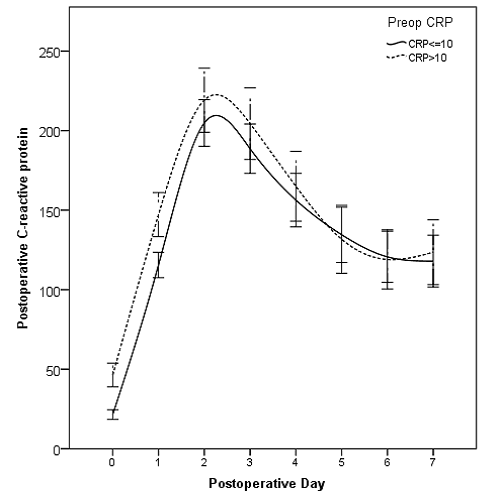
\includegraphics[width=\textwidth]{Figures/sirs_crp_crp}
		\caption{Preop. CRP vs. postop. CRP}
		\label{fig:sirs_crp_crp}
	\end{subfigure}
	\hfill
	\begin{subfigure}{0.48\textwidth}
		\centering
		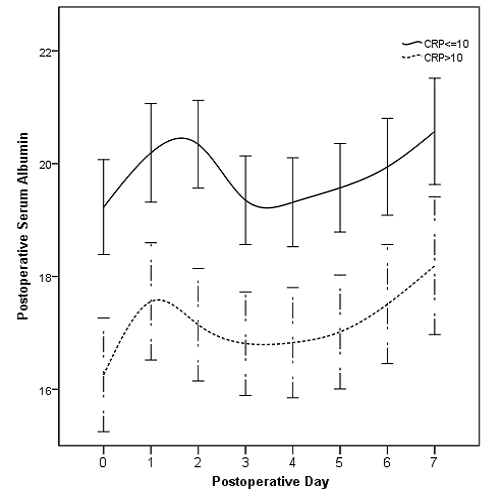
\includegraphics[width=\textwidth]{Figures/sirs_crp_alb}
		\caption{Preop. CRP vs. postop. Albumin}
		\label{fig:sirs_crp_alb}
	\end{subfigure}
	
	\begin{subfigure}{0.48\textwidth}
		\centering
		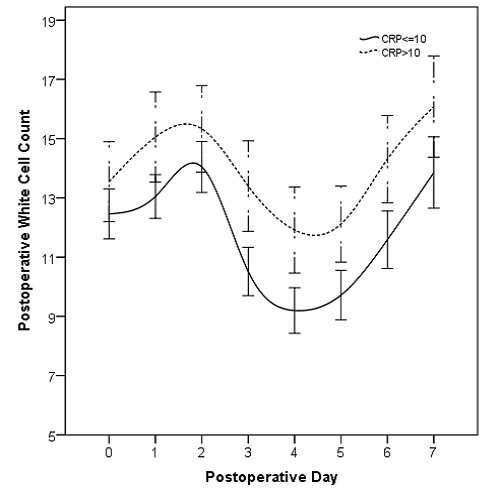
\includegraphics[width=\textwidth]{Figures/sirs_crp_wcc}
		\caption{Preop. CRP vs. postop. White Cell Count}
		\label{fig:sirs_crp_wcc}
	\end{subfigure}
	\hfill
	\begin{subfigure}{0.48\textwidth}
		\centering
		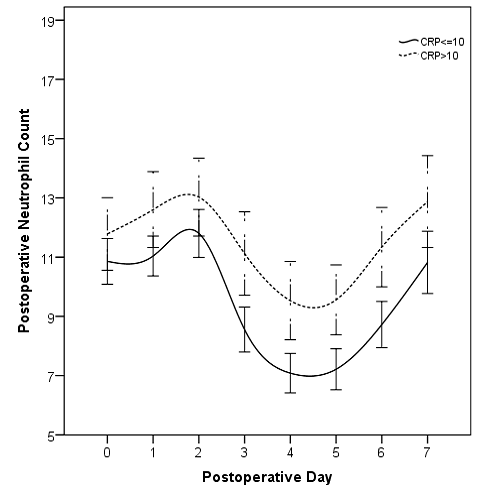
\includegraphics[width=\textwidth]{Figures/sirs_crp_neut}
		\caption{Preop. CRP vs. postop. Neutrophil Count}
		\label{fig:sirs_crp_neut}
	\end{subfigure}	
\end{figure}
%==============================================================================

%========================Albumin vs Post-op SIRS============================================
\clearpage
\begin{figure}[p]
	\caption{Relationship between preoperative Albumin levels and postoperative inflammatory markers in the first week after pancreaticoduodenectomy.}
	\label{fig:sirs_alb}
	\centering
	\begin{subfigure}{0.48\textwidth}
		\centering
		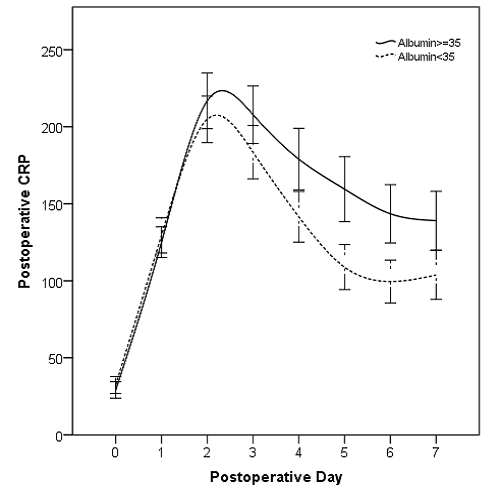
\includegraphics[width=\textwidth]{Figures/sirs_alb_crp}
		\caption{Preop. Albumin vs. postop. CRP}
		\label{fig:sirs_alb_crp}
	\end{subfigure}
	\hfill
	\begin{subfigure}{0.48\textwidth}
		\centering
		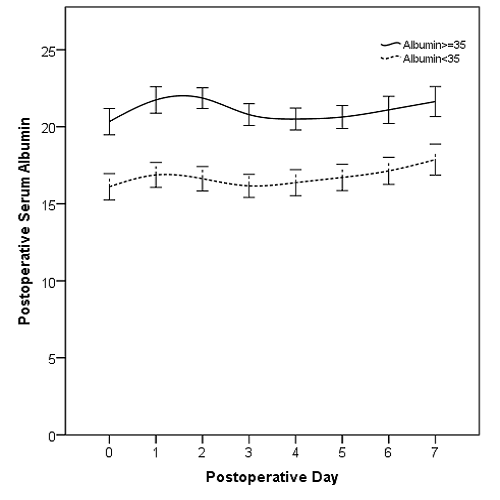
\includegraphics[width=\textwidth]{Figures/sirs_alb_alb}
		\caption{Preop. Albumin vs. postop. Albumin}
		\label{fig:sirs_alb_alb}
	\end{subfigure}
	
	\begin{subfigure}{0.48\textwidth}
		\centering
		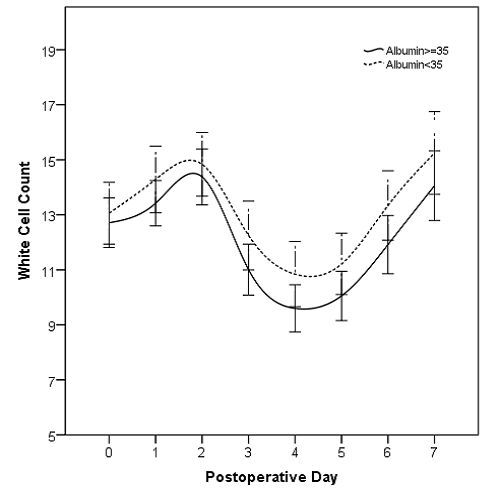
\includegraphics[width=\textwidth]{Figures/sirs_alb_wcc}
		\caption{Preop. Albumin vs. postop. White Cell Count}
		\label{fig:sirs_alb_wcc}
	\end{subfigure}
	\hfill
	\begin{subfigure}{0.48\textwidth}
		\centering
		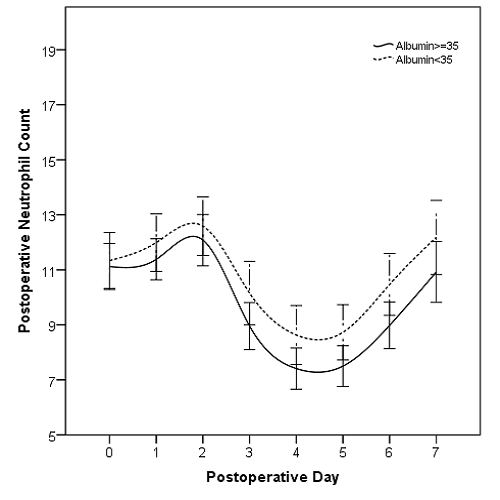
\includegraphics[width=\textwidth]{Figures/sirs_alb_neut}
		\caption{Preop. Albumin vs. postop. Neutrophil Count}
		\label{fig:sirs_alb_neut}
	\end{subfigure}	
\end{figure}
%==============================================================================

%========================Bilirubin vs Post-op SIRS============================================
\clearpage
\begin{figure}[p]
	\caption{Relationship between preoperative obstructive jaundice and postoperative inflammatory markers in the first week after pancreaticoduodenectomy.}
	\label{fig:sirs_bilirubin}
	\centering
	\begin{subfigure}{0.48\textwidth}
		\centering
		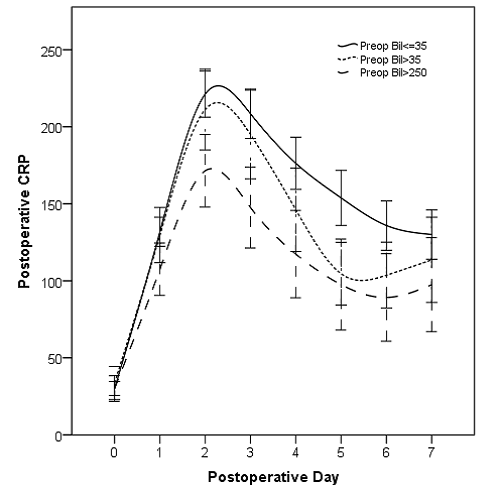
\includegraphics[width=\textwidth]{Figures/sirs_bil_crp}
		\caption{Preop. Bilirubin vs. postop. CRP}
		\label{fig:sirs_bil_crp}
	\end{subfigure}
	\hfill
	\begin{subfigure}{0.48\textwidth}
		\centering
		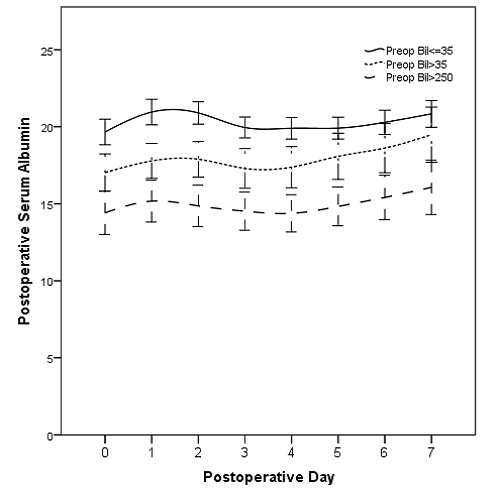
\includegraphics[width=\textwidth]{Figures/sirs_bil_alb}
		\caption{Preop. Bilirubin vs. postop. Albumin}
		\label{fig:sirs_bil_alb}
	\end{subfigure}
	
	\begin{subfigure}{0.48\textwidth}
		\centering
		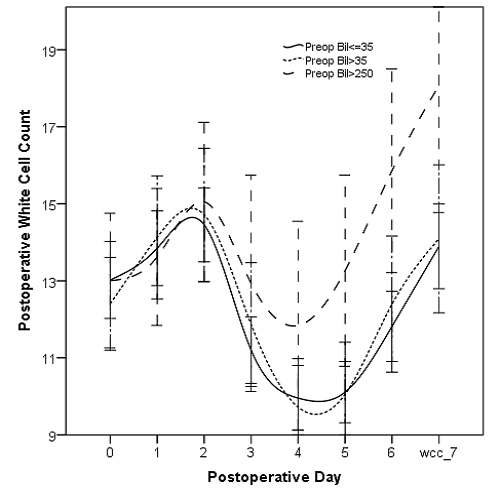
\includegraphics[width=\textwidth]{Figures/sirs_bil_wcc}
		\caption{Preop. Bilirubin vs. postop. White Cell Count}
		\label{fig:sirs_bil_wcc}
	\end{subfigure}
	\hfill
	\begin{subfigure}{0.48\textwidth}
		\centering
		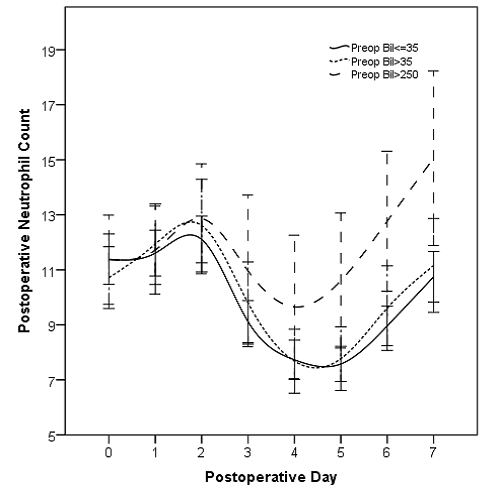
\includegraphics[width=\textwidth]{Figures/sirs_bil_neut}
		\caption{Preop. Bilirubin vs. postop. Neutrophil Count}
		\label{fig:sirs_bil_neut}
	\end{subfigure}	
\end{figure}
%==============================================================================
%\input{Tables/sirs_crp_bodycomp}

%========================Bilirubin vs Post-op SIRS============================================
\clearpage
\begin{figure}[p]
	\caption{Relationship between preoperative $\dot{V}_{O_2}$AT and postoperative inflammatory markers in the first week after pancreaticoduodenectomy.}
	\label{fig:sirs_at}
	\centering
	\begin{subfigure}{0.48\textwidth}
		\centering
		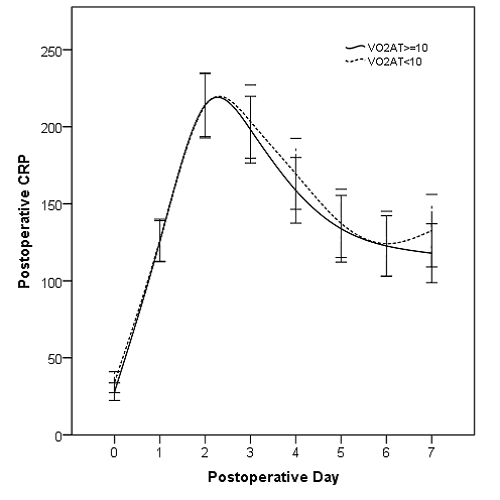
\includegraphics[width=\textwidth]{Figures/sirs_at_crp}
		\caption{Preop. $\dot{V}_{O_2}$AT vs. postop. CRP}
		\label{fig:sirs_at_crp}
	\end{subfigure}
	\hfill
	\begin{subfigure}{0.48\textwidth}
		\centering
		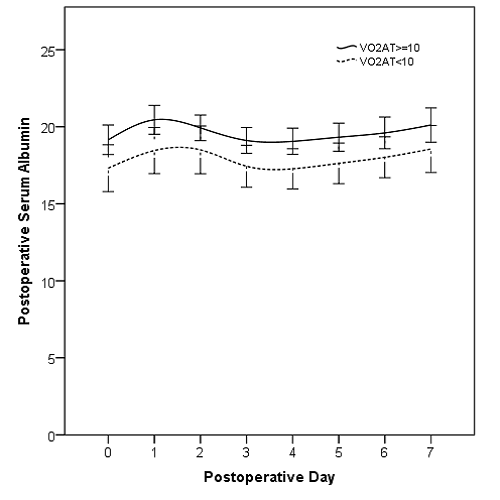
\includegraphics[width=\textwidth]{Figures/sirs_at_alb}
		\caption{Preop. $\dot{V}_{O_2}$AT vs. postop. Albumin}
		\label{fig:sirs_at_alb}
	\end{subfigure}
	
	\begin{subfigure}{0.48\textwidth}
		\centering
		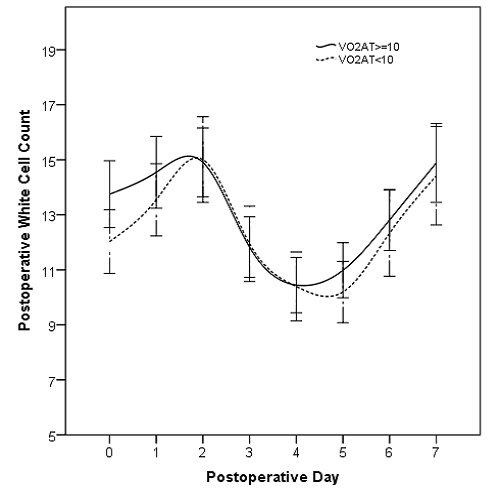
\includegraphics[width=\textwidth]{Figures/sirs_at_wcc}
		\caption{Preop. $\dot{V}_{O_2}$AT vs. postop. White Cell Count}
		\label{fig:sirs_at_wcc}
	\end{subfigure}
	\hfill
	\begin{subfigure}{0.48\textwidth}
		\centering
		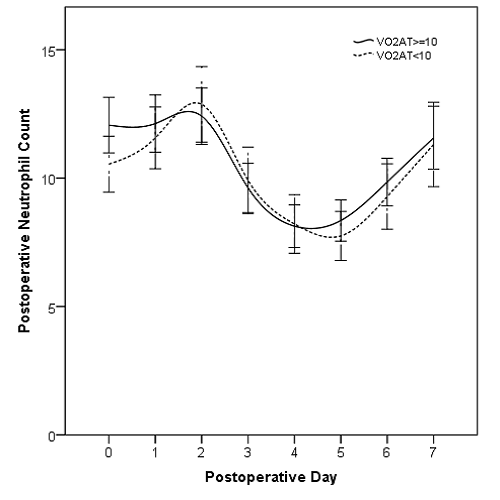
\includegraphics[width=\textwidth]{Figures/sirs_at_neut}
		\caption{Preop. $\dot{V}_{O_2}$AT vs. postop. Neutrophil Count}
		\label{fig:sirs_at_neut}
	\end{subfigure}	
\end{figure}
%==============================================================================


\section{Discussion}